\chapter{Numeric Models}
\label{chap:numeric}
In this chapter, the numeric theory behind the two models used to analyze the fatigue of the dynamic power cable is presented.

\section{The Finite Element Method}
The finite element method is a numerical procedure for solving differential equations and is often used in analyses of structures. The finite element method gives an approximate solution, with increasing accuracy with decreasing mesh size. According to the Finite Element Theory, for a static linear system, the system relationship is:
\begin{equation}
    \boldsymbol{R}= \boldsymbol{K}\boldsymbol{r}
\end{equation}
Where \textbf{R} is the global load matrix, \textbf{K} is the global stiffness matrix, and \textbf{r} is the nodal displacement vector.\newline
\newline
This is based on the following principles:
\begin{itemize}
    \item Equilibrium
    \item Kinematic compatibility
    \item Stress-strain relationship
\end{itemize}
 \cite{moan2003}
\subsection{Principle of Virtual Work}
The element stiffness relationship can be derived based on virtual work (Galerkin's Method). This method assumes a displacement for each element so that the displacement is continuous between elements. The method can be generalized and used for all kinds of structural problems in all dimensions, \cite{moan2003}. The method gives an approximation rather than the exact solution. This is done by, on average, fulfilling the differential equations in the problem. By setting the internal work equal to the external work, it is assumed that the error from assuming the weight function in the external work is equal to the error in the internal work. If the weight functions are selected so that the boundary conditions are fulfilled appropriately, the error in the external work will cancel out. This means that the total error in the volume integration is zero on average, but at an arbitrary point, the equilibrium equation is not necessarily fulfilled. This is referred to as integrated equilibrium. The principle of virtual work in a body with deformed volume and surfaces in equilibrium:   

\begin{equation}
    \int_v (\rho \boldsymbol{\ddot{u}} - \boldsymbol{f}) \cdot \delta \boldsymbol{u}dV + \int_V \boldsymbol{\sigma}: \delta \epsilon dV - \int_S \boldsymbol{t} \cdot \delta \boldsymbol{u} dS =0
    \label{eq:virtual}
\end{equation}
Where V refers to the volume, $\rho$ is the material density, $ \boldsymbol{\ddot{u}}$ is the acceleration field, $ \boldsymbol{f}$ is the volume force vector, $\delta$ is the virtual displacement,  $\boldsymbol{\sigma}$ is the stress tensor, $\epsilon$ is the natural strain tensor, $\boldsymbol{t}$ is the surface traction, $\boldsymbol{u}$ is the displacement vector and S refers to the surface \cite{Bflextheory2013}. 

\begin{comment}
In BFLEX and SIMA RIFLEX(?) the stress tensor is given as: 
\begin{equation}
\boldsymbol{S}=\frac{\rho_0}{\rho} \boldsymbol{F^{-1}} \cdot \boldsymbol{\sigma} \cdot \boldsymbol{F}
\end{equation}
Where $\rho_0$ is the density of the material in the initial configuration, and $\rho$ is the density of the material in the deformed configuration, $\boldsymbol{F}$ is the deformed gradient. In this case, strains are usually small so that $\boldsymbol{S}$ and $\boldsymbol{\sigma}$ can be treated equally. However, equation \ref{eq:virtual} need to be modified as change of are will affect pressure loads. The equation then becomes:

\begin{equation}
    \int_v (\rho \boldsymbol{\ddot{u}} - \boldsymbol{f}) \cdot \delta \boldsymbol{u}dV_0 + \int_V \boldsymbol{\sigma}: \delta \epsilon dV_0 - \int_S \boldsymbol{t} \cdot \delta \boldsymbol{u} dS_0 -  \int_S \boldsymbol{p} \cdot \delta \boldsymbol{u}(1+\epsilon_{11} + \epsilon_{33})  dS_0 =0
    \label{eq:virtual2}
\end{equation}
Where $\epsilon_{11}$ and $\epsilon_{33}$ are principle strains of surface plane.
\end{comment}
\section{Method for Static calculation}
\subsection{Static Non-linear Theory}
According to \cite{moan2003}, a system is non-linear if it contains non-linear material, large displacements or geometry non-linearity. For non-linear problems, the stiffness will depend on the displacement:
\begin{equation}
    \boldsymbol{R}=\boldsymbol{K(r)}\boldsymbol{r}
\end{equation}
The stiffness matrix is often written on differential form, with the incremental stiffness matrix, $K_I$:
\begin{equation}
    d\boldsymbol{R}=\frac{d}{d\boldsymbol{r}}(\boldsymbol{K(r)r})d\boldsymbol{r}
\end{equation}
\begin{equation}
  d\boldsymbol{R}= \boldsymbol{K_I(r)}d\boldsymbol{r}
  \label{eq:system}
\end{equation}
In general it can be challenging to determine $\boldsymbol{r}$ for a given $\boldsymbol{R}$ analytically, and thus iterative methods will have to be used. Only the methods relevant for this project will be presented here. 

\subsection{Combined Method}
The combined method is a combination of the Euler-Cauchy Method and the Newton-Raphson Method. 
\subsubsection{Euler-Cauchy Method}
This method it an incremental method, meaning that the external load is applied step-wise. For each step the displacement increment $\boldsymbol{\Delta r}$ is determined. The total displacement is then calculated by adding the incremental displacements. The incremental stiffness matrix $\boldsymbol{K_I}$ is constant for each increment, and is calculated for each step based on the current displacement and stress before a new load increment is added. This is illustrated in Figure \ref{fig:euler}. For load increment number (m+1):
\begin{equation}
\Delta \boldsymbol{r_{m+1}}= \boldsymbol{K_{I}}(\boldsymbol{r_{m}})^{-1} \Delta \boldsymbol{R_{m+1}}
\end{equation}
\newline 
\newline
where:
\begin{equation}
    \Delta \boldsymbol{R_{m+1}} = \boldsymbol{R_{m+1}} - \boldsymbol{R_{m}}
\end{equation}
\begin{equation}
    \boldsymbol{r_{m+1}}=\boldsymbol{r_{m}}+\Delta \boldsymbol{r_{m+1}}
\end{equation}

\begin{figure}[H]
\centering
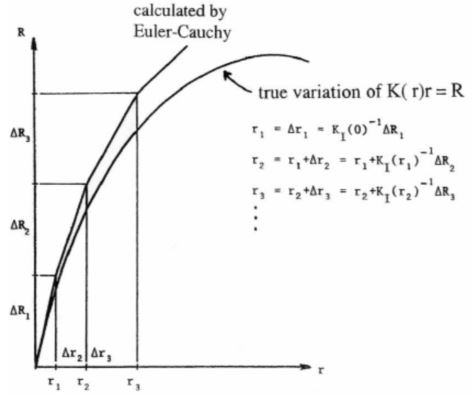
\includegraphics[scale=1]{figures/euler}
\caption[$\; \:$Euler-Cauchy Method]{Euler-Cauchy Method, \cite{moan2003} }
 \label{fig:euler}
\end{figure}
\noindent As the incremental stiffness from the previous increment is used, this will only give an approximation, and does not fulfill total equilibrium. This can be seen in Figure \ref{fig:euler} where the approximation is plotted with the true solution. More accurate results will be obtained by using smaller increment size and by equilibrium corrections. 
\subsubsection{Newton Raphson Method}
\label{sec:newton}
The Newton-Raphson Method is an iterative method, and is based on the Newton-Raphson Algorithm:
\begin{equation}
    x_{n+1}=x_n - \frac{f(x_n)}{f'(x_n)}
\end{equation}
 Where $f'(x_n)$ is the derivative of $f(x)$ at $x=x_n$. This is illustrated in Figure \ref{fig:newton}
 \noindent This algorithm can be generalized to solve the non-linear system equation \ref{eq:system}:
 \begin{equation}
  \boldsymbol{r_{n+1}}= \boldsymbol{r_n-K_I^{-1}(r_n)(R_{int}-R)} 
\end{equation}
This method requires that $\Delta r_{n+1}$ is solved for from 
\begin{equation}
   \boldsymbol{R-R_{int}}=\boldsymbol{K_{I(n)}\Delta r_{n+1}}
   \label{eq:newton}
\end{equation}
and that $K_I$ is established. 
 \begin{figure}[H]
\centering
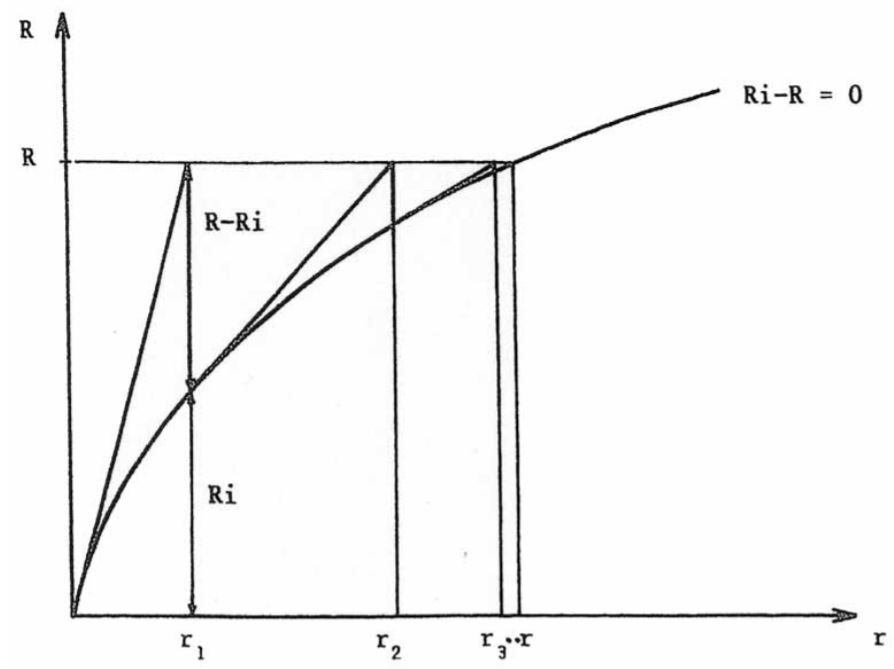
\includegraphics[scale=0.5]{figures/newton2}
\caption[$\; \:$Newton-Raphson Iteration]{Newton-Raphson Iteration, \cite{moan2003} }
 \label{fig:newton}
\end{figure}
\noindent Newton-Raphson method is time consuming, but calculation time can be improved by updating $\boldsymbol{K_I}$ less frequently. That is called the modified Newton-Raphson method, and usually gives slower convergence.  The iteration ends when the displacement from one iteration to the next is smaller than the convergence criteria:
\begin{equation}
    ||\boldsymbol{r_{n+1}-r_n||} < \epsilon
\end{equation}

\subsubsection{Combined Method}
\label{sec:combined}
When combining the two methods load is applied according to the Euler-Cauchy method, and iteration until equilibrium is done according to the modified Newton-Raphson method for each increment as illustrated in Figure \ref{fig:combined} The method is considered to be effective as long as the load curve is increasing with displacement. For extremal points in the load-displacement curve, additional procedures need to be implemented.    

 \begin{figure}[H]
\centering
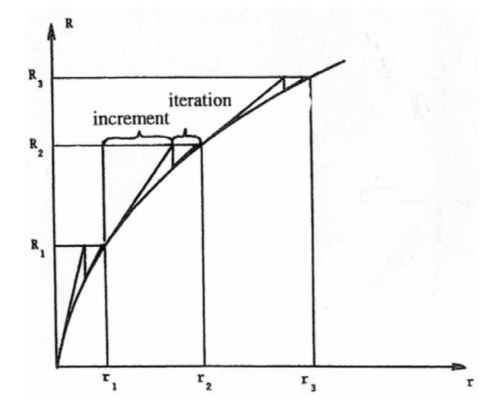
\includegraphics[scale=0.8]{figures/combined}
\caption[$\; \:$Combined Method]{Combined Method, \cite{moan2003} }
 \label{fig:combined}
\end{figure}
\section{Method for Dynamic Calculation}
Dynamic analysis has to be considered when external loads are not applied in a very slow manner. Dynamic loads are different from static loads by implying a time dependent solution and by introducing inertia loads throughout the structure, and often also damping. The equilibrium equation for a dynamic system is stated by \cite{Langen1999} as:

\begin{equation}
  \boldsymbol{M \ddot{r}} + \boldsymbol{C \dot{r}} + \boldsymbol{Kr} =  \boldsymbol{Q}(t)
  \label{eq:eq}
\end{equation}

\noindent A variation of Equation \ref{eq:eq} is the semi-discrete global equation describing the instantaneous equation of motion of a non-linear system at time t. This relation is presented by \cite{Mathisen1990} as:
\begin{equation}
    \boldsymbol{R^I}+ \boldsymbol{R^D} + \boldsymbol{R^S}=\boldsymbol{R^E}
\end{equation}
Where $\boldsymbol{R^I}$ is the inertia force vector, $\boldsymbol{R^D}$ is the damping force vector, $\boldsymbol{R^S}$ is the internal force vector and $\boldsymbol{R^E}$ is the external force vector. \newline
\newline
The inertia forces relate to the mass matrix as:
\begin{equation}
    \boldsymbol{R^I}= \boldsymbol{R^I(\ddot{r},\dot{r},r,}t)=\boldsymbol{M(\ddot{r},\dot{r},r,}t)\boldsymbol{r}
\end{equation}

\noindent The internal forces $\boldsymbol{R^S}$ can be established by:
\begin{equation}
    \frac{\partial \boldsymbol{R^S} }{\partial\boldsymbol{r}}= \boldsymbol{K^M}+\boldsymbol{K^G}
\end{equation}
\noindent The total tangential stiffness is now:
\begin{equation}
    \boldsymbol{K^_T}=\boldsymbol{K_T(\ddot{r},\dot{r},r},t)=\boldsymbol{K^M}+\boldsymbol{K^G}+\boldsymbol{K^{NC}}
\end{equation}
\begin{equation}
    \boldsymbol{K^{NC}}=\boldsymbol{K^{NC}(\ddot{r},\dot{r},r},t)=  \frac{\partial \boldsymbol{R^{NC}} }{\partial\boldsymbol{r}}
\end{equation}
\noindent Where $\boldsymbol{K^M}$ and $\boldsymbol{K^G}$ are the material and geometric stiffness matrices respectively, and $\boldsymbol{K^{NC}}$ is the total external non-conservative external forces. \newline
\newline
The equivalent damping force can be expressed as:
\begin{equation}
    \boldsymbol{R^_D}=\boldsymbol{R_D(\ddot{r},\dot{r},r},t)=  \boldsymbol{C_T}\boldsymbol{\dot{r}}
\end{equation}
And the tangential damping matrix is:
\begin{equation}
      \boldsymbol{C_{T}}=\boldsymbol{C_T(\ddot{r},\dot{r},r,}t)=\alpha_1 \boldsymbol{M}+\alpha_2\boldsymbol{K_T} + C_d 
\end{equation}
Where $\alpha_1$ and $\alpha_2$ are the damping coefficients for the Rayleigh damping and $C_d$ is the damping coefficient matrix for additional discrete nodal points.  
\newline
\newline 
\noindent  The dynamic equilibrium equation is an initial value problem, meaning that start values determine the solution. Practical numerical integration methods use a step-by-step approach, where the time interval is divided into sub-intervals with step length h. Displacement, velocity, and acceleration are known for the beginning of the sub-interval, and the solution for the end of the sub-interval is calculated by assuming the variation of the acceleration over the time step. The computed value is used to determine the velocity and displacement across the time step, and they are the start values for the next sub-interval. This way, an approximated solution is calculated at instants along the time axis, and accuracy increases as h decreases, \cite{Langen1999}.
\newline 
\newline
 \noindent How the acceleration changes during a time step is suggested by several methods and can be explicit or implicit. A non-linear implicit method requires iteration at each time step to establish for each time step, while this is not necessary for an explicit method. Only the methods relevant to this master thesis are presented\newline
 \newline
\noindent 
\subsection{Newmark's $\boldsymbol{\beta}$ Family}
\label{sec:newmark}
Newmark-$\boldsymbol{\beta}$ is a family of numerical integration of the dynamic equilibrium equations. It can easily be derived from assuming a constant average acceleration over the time step. The following equations are taken from \cite{sintef2017} and \cite{Mathisen1990}: 
\begin{equation}
   \boldsymbol{M_t \ddot{r}_{t+\Delta t}} + \boldsymbol{C_{T,t}\dot{r}_{t+\Delta t}} + \boldsymbol{R_{t+\Delta t}^S}=\boldsymbol{{R_{t+\Delta t}^E}}
   \label{eq:new}
\end{equation}
\begin{equation}
    \boldsymbol{\dot{r}_{t+\Delta t}} =\boldsymbol{\dot{r}_{t}}+(1-\gamma)\boldsymbol{\ddot{r}_{t}}\Delta \tau + \gamma \boldsymbol{\ddot{r}_{t+\Delta t}} \Delta \tau
\end{equation}
\begin{equation}
    \boldsymbol{r_{t+\Delta t}} =\boldsymbol{r_{t}}\Delta \tau + (\frac{1}{2}-\beta)\boldsymbol{\ddot{r}_{t}}(\Delta \tau)^2 + \beta \boldsymbol{\ddot{r}_{t+\Delta t}} (\Delta \tau)^2
\end{equation}
where  $\Delta \tau =\theta \Delta t, \leq 1.0$\newline
\newline
$\gamma$ and $\beta$ are parameters defining the change in acceleration, velocity and displacement vectors in time step $\Delta t$. \cite{Langen1999} explains that the equations are obtained from Taylor-series expansion.  Different values of these parameters give different methods in the Newmark-$\boldsymbol{\beta}$ family. $\gamma$ represents the numerical damping, taken from \cite{sintef2017}: 
\begin{itemize}
    \item $\gamma > \frac{1}{2}$: Positive numerical damping
    \item $\gamma < \frac{1}{2}$: Negative numerical damping
    \item $\gamma = \frac{1}{2}$: No numerical damping
\end{itemize}

\noindent $\gamma = \frac{1}{2}$ is customarily used to assure second order accuracy and stability. 
According to \cite{Mathisen1990}, the Newmark-$\boldsymbol{\beta}$ method may have difficulties with solving non-linear problems if they are not discretized in the right way. \newline
\newline
\noindent In dynamic analysis, the higher modes are of little interest, and these can be removed by introducing an increased damping ratio. The Newmark's $\boldsymbol{\beta}$ Family removes the medium modes, and not affecting the lowest and highest modes. The higher modes can be removed by introducing numerical damping, but it is at the cost of accuracy.  The method can be applied both for linear and non-linear analysis \cite{sintef2017}.

\subsection{Modified Hilber-Hughes-Taylor Method}
\label{sec:HHT}
The problem with accuracy when removing the higher modes can be fixed by using Hilber-Hughes-Taylor Method, often referred to as HHT-$\alpha$. The method maintains accuracy while introducing artificial damping of the higher modes. This is done through the modification of equation \ref{eq:new}. 
\begin{equation}
\begin{split}
   \boldsymbol{M_t \ddot{r}_{t+\Delta t}} + (1+\alpha_H)\boldsymbol{C_{T,t}\dot{r}_{t+\Delta t}}  -\alpha_H\boldsymbol{C_{T,t}\dot{r}}_{n}+ (1+\alpha_H)\boldsymbol{R_{t+\Delta t}^S}-\alpha_H\boldsymbol{R_{t}^S}\\=(1+\alpha_H) \boldsymbol{R_{t+\Delta t}^E}-\alpha_H\boldsymbol{R_{t}^E}
   \end{split}
\end{equation}

The method is unconditionally stable when:
\begin{itemize}
    \item $-\frac{1}{3} \leq \alpha_H \leq 0 $
    \item  $\gamma = \frac{1}{2} (1-2 \alpha_H)$
    \item  $\beta = \frac{1}{4} (1- \alpha_H)^2$
\end{itemize}

\noindent The method is effectively suppressing high frequency and also retains second-order accuracy, \cite{Mathisen1990}.

\section{Global Model in SIMA RIFLEX}
SIMA RIFLEX is a computer program made for analyzing slender structures such as flexible risers and mooring lines developed by SINTEF Ocean. The Combined Method is used for the static calculation, and Newmark-$\boldsymbol{\beta}$ is used for dynamic analysis. These methods are described in section \ref{sec:combined} and \ref{sec:newmark} respectively. 


\subsection{Element Formulation}
\label{sec:ghost}
SIMA RIFLEX uses co-rotated ghost reference as element formulation for beam elements. 
\begin{comment}
\subsection{Total Lagrangian Formulation}
\label{sec:ghost}
For non-linear analysis, an incremental approach is necessary as described above. According to \cite{sintef2017}, the initial configuration of the body, C0, and the deformed Cn at time t, and then the new incremental deformation Cn+1 at t+$\Delta$t. Cn+1 is similar to Cn, as $\Delta$t is small. This formulation where the strains in all the incremental configurations are referred to the initial configuration is called "Total Lagrangian Formulation." \cite{Mathisen1990} states that this method can produce false straining in beam elements when exposed to large rotations, and should thus only be used for small rotations
\subsubsection{Co-Rotated Ghost Reference}
\label{sec:ghost}
\end{comment}
Co-rotated beam elements use Green strain and 2nd
Piola-Kirchhoff stresses as the Total Lagrangian formulation, but adapts the procedure of Updated Lagrange formulation where the configuration is updated. This yields the following stiffness matrix:
\begin{equation}
    \boldsymbol{K_I}= \boldsymbol{K_0} + \boldsymbol{K_\sigma}
\end{equation}
This is convenient when it is assumed that the initial configuration deforms as a rigid body, and will move and rotate with the motion of the body. At any time the initial configuration is close to the deformed configuration, \cite{sintef2017}. \cite{Mathisen1990} explains that each beam element has a local coordinate system, $i_i^0$ as illustrated in Figure \ref{fig:coro} where the initial configuration $C_0$ moves as a rigid body with the element and becomes $C_{0n}$. The deformed beam element will have its local coordinate system rotated, now denoted $i_ia$ and $i_i^b$. This forms the reference for the calculation of stresses and strains. 

\begin{figure}[H]
\centering
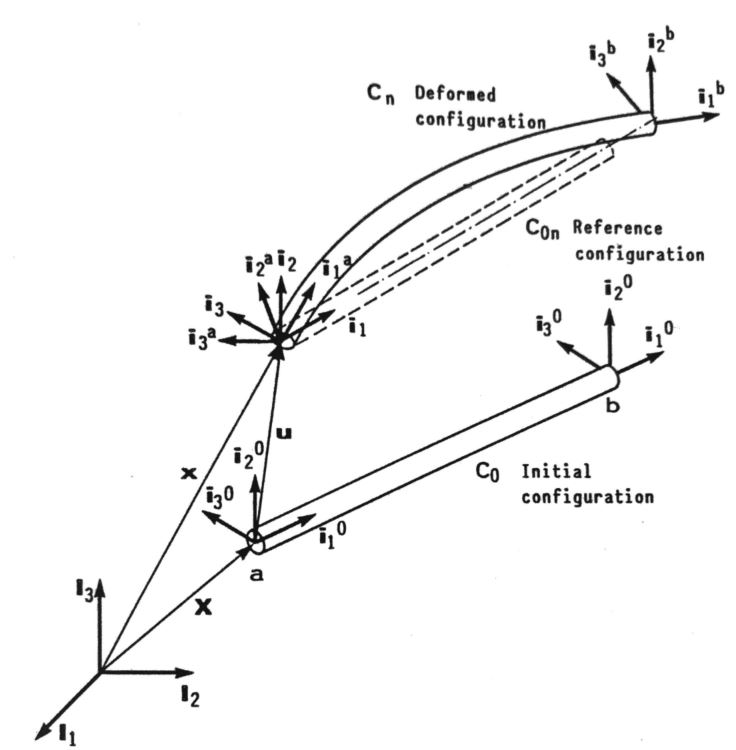
\includegraphics[scale=0.5]{figures/coro}
\caption[$\; \:$Co-rotated Ghost Reference]{Co-rotated Ghost Reference, \cite{Mathisen1990} }
 \label{fig:coro}
\end{figure}

\subsection{Element Description}
In this section, the relevant element type and its kinematics are presented. Only the element used in the master thesis is included. 
\subsubsection{Beam element}
\noindent The beam element in SIMA RIFLEX has 2 nodes with 6 degrees of freedom for each node, 3 translational and 3 rotational that can be seen in Figure \ref{fig:beamri} that are defined in relation to the local Cartesian coordinate system in the initial C0n configuration,
\cite{sintef2017}.

\begin{figure}[H]
\centering
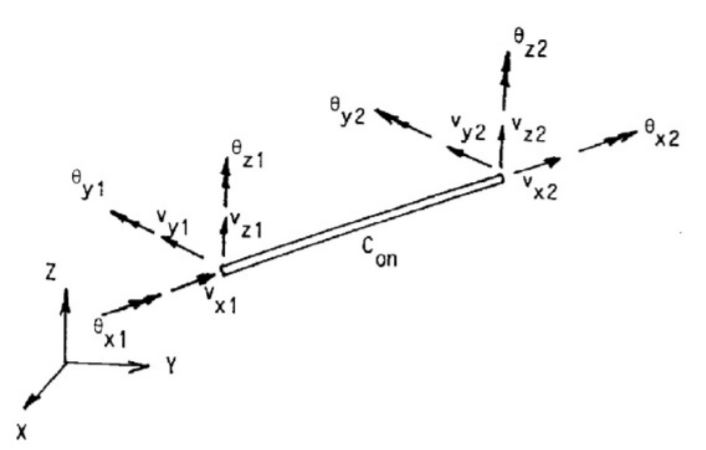
\includegraphics[scale=0.5]{figures/beamri}
\caption[$\; \:$Beam Element]{Degrees of freedom for the beam element, \cite{sintef2017} }
 \label{fig:beamri}
\end{figure}

\noindent \cite{sintef2017} states that it is assumed that straight lines normal to the midplane will remain straight and normal to the midplane, and that strains are small in the element in accordance with the Kirchhoff hypothesis.\newline
\newline The displacement of an arbitrary point, P with coordinates x,y, and z can be expressed as the following:
\begin{equation}
    u(x,y,z)=u_0(x) - y \frac{dv_0}{dx} - z \frac{dw_0}{dx}
\end{equation}
\begin{equation}
    v(x,y,z)=v_0(x) - z \theta
\end{equation}
\begin{equation}
    w(x,y,z)=w_0(x) + y \theta
\end{equation}


\subsection{Load Model}
The loads on the global model are mainly tension due to inertia and weight as well as external loads due to irregular waves. The theory in this section is mostly taken from \cite{sintef2017}.\newline
\newline
\noindent The inertia forces consist of:
\begin{equation}
    \boldsymbol{R^I(r,\dot{r}})= [\boldsymbol{M^S} + \boldsymbol{M^F(\dot{r})} + \boldsymbol{M^H (\dot{r})} ]\boldsymbol{\ddot{r}}
\end{equation}
Where $\boldsymbol{M^S}$ is the structural mass matrix, $\boldsymbol{M^F}$ is internal flow mass matrix, $\boldsymbol{M^H}$ is hydrodynamic mass matrix. 
\newline
\newline
\noindent The damping forces consists of:
\begin{equation}
    \boldsymbol{R^D(r,\dot{r}})= [\boldsymbol{C^S(r)} + \boldsymbol{C^H(r)} + \boldsymbol{C^D (r,\dot{r})} ]\boldsymbol{\dot{r}}
\end{equation}
Where $\boldsymbol{C^S}$ is the  internal structural damping matrix, $\boldsymbol{C^H}$ is hydrodynamic damping matrix, $\boldsymbol{C^D}$ is matrix of specified discrete dashpot dampers. \newline
\newline
\noindent The external load vector consists of:
\begin{itemize}
\item Weight and buoyancy.
\item Forced displacements due to support vessel movements.
\item Wave and particle accelerations in accordance to Morison's Equation, (see Equation \ref{eq:morison}).
\end{itemize}
In SIMA RIFLEX the water velocity and motion are decomposed into x,y and z, where x is in the longitudinal direction and y and z as the symmetry axes for the cross section.

\section{Local Model in BFLEX }
BFLEX is a computer program developed by Professor Svein Sævik. \cite{Bflextheory2013}  and \cite{Bflextheory2017} are used as a basis for this section.  The Newton-Raphson method, described in section \ref{sec:newton}, is used for calculations in the static analysis. While for the dynamic analysis, the modified HHT-$\alpha$ method described in section \ref{sec:HHT} is used.

\subsection{Element Formulation}
BFLEX also uses co-rotated ghost reference described in section \ref{sec:ghost}, 
where small strains are assumed, but at the same time allowing large rigid body motions due to a 4 base vector system. \\\\By looking at equation \ref{eq:virtual} for an infinite small increment, $\Delta$, and only including static terms the following is obtained: 
 \begin{equation}
    \int_V \boldsymbol{C}: (\epsilon + \Delta \boldsymbol{E}) : \delta (\epsilon + \Delta \boldsymbol{E})dV_0 - \int_S (\boldsymbol{t} + \Delta \boldsymbol{t}) \cdot \delta \boldsymbol{u} dS_0 =0
\end{equation}
 This is used as a basis for the stiffness matrix in BFLEX.
 
\begin{comment}
 \begin{equation}
    \int_V \boldsymbol{C}: \Delta \epsilon: \delta \epsilon dV_0 + \int_V \boldsymbol{\sigma}: \delta \Delta \boldsymbol{E} dV_0 \int_S \Delta \boldsymbol{t} dS_0 =0
\end{equation}
Where $\boldsymbol{E}$ is the Green strain tensor. By subtracting \ref{eq:virtual2} from \ref{eq:virtual} and assuming small difference in equilibrium state between two neighbouring elements and neglecting second order effects in $\Delta$, the following is obtained:
\end{comment}

\subsection{Element Descriptions}
\label{sec:el}
In this section, the relevant elements and their kinematics are described.
\subsubsection{PIPE31}
PIPE31 is an elastic element with two nodes and six degrees of freedom in each node. The following stresses are according to Hooke's law:
\begin{equation}
    \begin{bmatrix}
       \sigma_{11}\\[0.3em]
       \sigma_{22}\\[0.3em]
        \tau\\[0.3em]
     \end{bmatrix}= \frac{E}{1-\nu^2}  \begin{bmatrix}
       1 & \nu & 0           \\[0.3em]
       \nu & 1      & 0 \\[0.3em]
       0           & 0& \frac{1-\nu^2}{2(1+\nu)}
     \end{bmatrix} \begin{bmatrix}
       \epsilon_{11}\\[0.3em]
       \epsilon_{22}\\[0.3em]
        \gamma\\[0.3em]
     \end{bmatrix}
\end{equation}
The displacement of an arbitrary point p defined by the local coordinates in the cross section can be expressed as:
\begin{equation}
    u_1(x,y,z)=u_{1,0}-yu_{2,0}-zu_{3,0}
\end{equation}

\begin{equation}
    u_2(x,y,z)=u_{2,0}-z\theta_x
\end{equation}

\begin{equation}
    u_3(x,y,z)=u_{3,0}-y\theta_x
\end{equation}
\noindent Where $\sigma_{ij}$ is the stress in i,j direction, E is Young's modulus for the material, $\nu$ is the Poisson's number, $\epsilon_ij$ is the strain in i,j direction, $\gamma$ is the shear strain, $u_i$ is the displacement in i direction, and $\theta$ is the torsion.  
\subsubsection{HSHEAR353}
Helix beam element with 4 nodes; 2 centroid nodes, and 2 helix nodes. The nodal points have to be defined in polar coordinates. There are 24 active degrees of freedom in the element where 12 are connected to the standard beam degrees of freedom to describe the global strain quantities, and 12 degrees of freedom are used to describe the local displacement of the wire relative to the core as shown in Figure \ref{fig:353} . Due to this, cubic interpolation is possible in all directions, and membrane locking due to curvature coupling is avoided. The torsion DOF at the helix nodes are not yet activated because of kinematic constraints, and always have to be suppressed when using the element.

\begin{figure}[H]
\centering
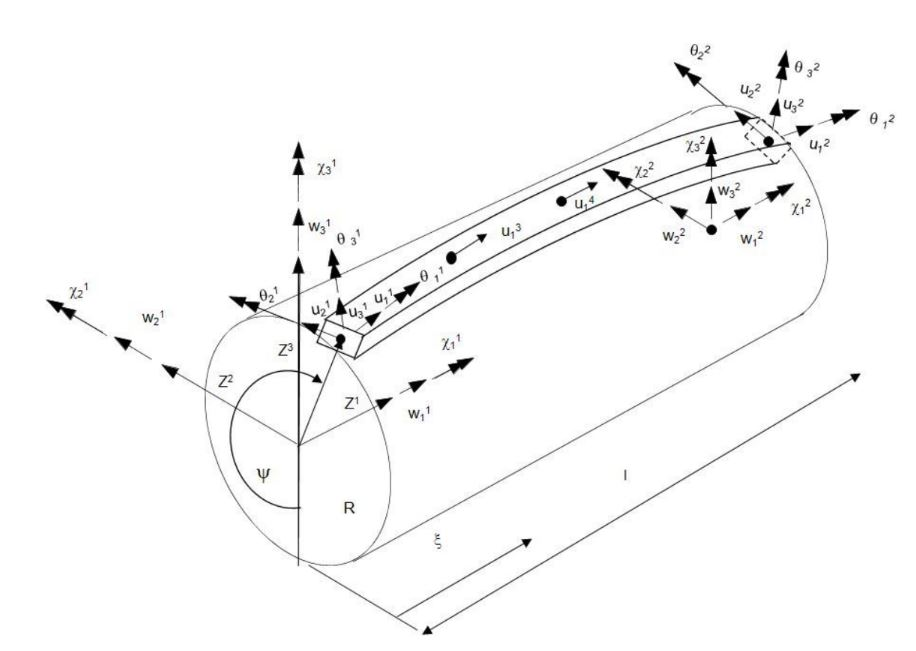
\includegraphics[scale=0.5]{figures/hshear353}
\caption[$\; \:$HSHEAR353]{Degrees of freedom for HSHEAR353 element, \cite{Bflextheory2013} }
 \label{fig:353}
\end{figure}


The strains can be described as:
\begin{equation}
    \epsilon_1=u_{1,1}-\kappa_3 u_2 + \kappa_2 \u_3
\end{equation}

\begin{equation}
    \epsilon_2=u_{2,1}-\kappa_3 u_1 + \kappa_1 \u_3
\end{equation}

\begin{equation}
    \epsilon_3=u_{3,1}-\kappa_2 u_1 + \kappa_1 \u_2
\end{equation}

The rotations can be expressed as:
\begin{equation}
    \omega_1=\kappa_1u_{1,1}-\kappa_t u_2,1 +\kappa_3(u_{3,1} + \kappa_1 u_2) + \kappa_2(u_{2,1}-\kappa_1 u_3 + \omega_{1p})
\end{equation}

\begin{equation}
    \omega_2=u_{3,11}-\kappa_2 u_1,1 -2\kappa_1u_{2,1} - \kappa_3 \kappa_t u_2 + \kappa_1 \kappa_1 u_{3} + \omega_{2}
\end{equation}

\begin{equation}
    \omega_3=u_{2,11}-\kappa_3 u_1,1 -2\kappa_1u_{3,1} - \kappa_2 \kappa_t u_2 + \kappa_1 \kappa_1 u_{2} + \omega_{3}
\end{equation}

\noindent Where $u_{i,j}$ is the differentiation of the displacement $u_i$ along the axis $X^i$ with respect to the curve linear coordinate $X^j$. $\epsilon_1$, $\epsilon_2$ and $\epsilon_3$ are the axial strain, the center line rotation about the $X^3$ axis and the center line rotation about the $X^2$ axis respectively. $\omega_1$, $\omega_2$ and $\omega_3$ are the center line torsion, the curvature about the $X^3$ axis and the curvature about the $X^2$ axis respectively. The $\omega_ip$ are the prescribed torsion and curvatures, and the $\kappa_i$ represents the initial torsion and curvatures. $\chi_i$ is prescribed rotation quantities at the pipe centerline and $\kappa_t$ is given as:
\begin{equation}
    \kappa_t=\frac{\cos^2\alpha}{R}+\sin^2 \alpha (\frac{-w_{2,11}\sin \psi }{1-R w_{2,11} \sin \psi} + \frac{w_{3,11}\cos \psi }{1+R w_{3,11} \cos \psi}
\end{equation}

\subsubsection{HSHEAR363}
Helix beam element with 3 nodes; 2 centroid nodes and 1 radial node to describe the radial motion. The centroid nodes have 6 degrees of freedom each and take care of the axial and torsional stiffness, while the radial node has 1 degree of freedom to be able to describe the radial motion and take care of circumferential strain.  The nodal points can be described with Cartesian coordinates. It can be interpreted as a simplified shell, and the aim for this element is to describe plastic layers, tape layers, and pressure armor. The degrees of freedom for the HSHEAR363 element are displayed in Figure \ref{fig:363}. 

\begin{figure}[H]
\centering
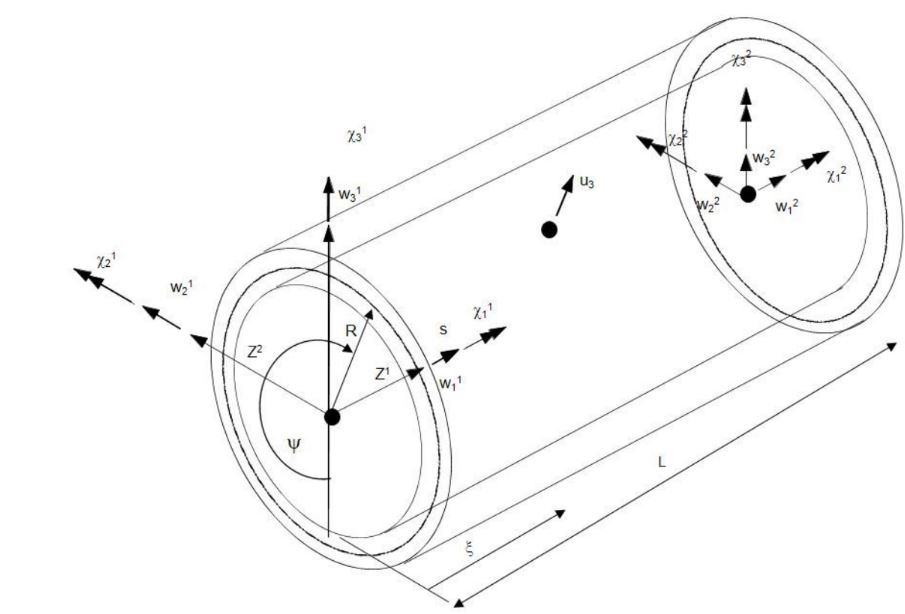
\includegraphics[scale=0.5]{figures/hshear363}
\caption[$\; \:$HSHEAR363]{Degrees of freedom for HSHEAR363 element, \cite{Bflextheory2013} }
 \label{fig:363}
\end{figure}

\noindent The radial displacement can be described as:
\begin{equation}
    u_3=(\gamma_1 + \gamma_2 \cos 2 \psi + \gamma_3 \sin2 \psi)
\end{equation}
\noindent For pressure armour and tape layers the longitudinal strain can be described as:

\begin{equation}
    \epsilon_{11}=cos^2 \alpha w_{1,1} + \frac{\sin^2 \alpha}{R} u_3 + R \sin \alpha \cos \alpha \chi_{1,1}-u_{3,22} \sin^2 \alpha X^3
\end{equation}
While for the plastic layer the strains can be described as:
\begin{equation}
    \epsilon_{11}=w_{1,1} + w_{3,11}R \cos \psi - w_{2,11}R \sin {\psi}
\end{equation}

\begin{equation}
    \epsilon_{22}=\frac{u_3}{R}-u_{3,22} X^3
\end{equation}

\begin{equation}
    \epsilon_{12}=R\chi_{1,1}
\end{equation}

\subsubsection{HCONT463}
HCONT463 was used to model contact between different layers in a cross-section.  Considering two different bodies, A and B where a is inside B. The HCONT463 is made to match the quantities of the HSHEAR353 and the HSHEAR363 elements. For the HSHEAR363 element, the radial displacement is considered only, while for HSHEAR353, the longitudinal and transverse direction are included. Figure \ref{fig:HCONT463} shows the element connecting a HSHEAR353 element and a HSHEAR363 element. The HSHEAR353 side includes 10 DOFs while the HSHEAR363 side includes 3 DOFs resulting in 13 nodes in total. The element is in reality equipped with 15 DOFs where the torsion DOFs are dummies.\\\\ When the element is used, it is important to begin in the inner layer of the cross-section. This element begins as the master element and connects its radial node nodes to the two radial nodes of the slave element. Then the slave element becomes the master element and connects its two radial nodes to the radial node of the element on the outside again, until the outer layer is reached.\\\\The energy functional $\Delta \pi$ is can be described as:
\begin{equation}
    \Delta \pi = \sum_{l=A}^B \Delta \bar{\pi}^{l} - \int_{S_c} (\lambda_n + \Delta \lambda_n) \cdot gds - \frac{1}{2 \alpha} \int_{S_c} \Delta \lambda_n^2 ds - \int_{S_c} \lambda_t \cdot \Delta \gamma ds - \frac{1}{2} \int_{Sc} \Delta \lambda_t \Delta \gamma ds
    \label{eq:energy}
\end{equation}
where $\Delta \bar{\pi}^{l}$ is the incremental potential of the bodies of A and B, $\lambda_t$ is the shear stress, $\lambda_n$ is can be found from equation \ref{eq:contact}, $\alpha$ is a scaling parameter related ot the surface stiffness. \\\\ To fulfill equilibrium for the two bodies on the time interva $[t,t+\Delta t]$ it is necessary that:
\begin{equation}
    \delta \Delta \pi =0
\end{equation}
In addition to the traditional Euler equations and boundary conditions the following constraint condition is recovered: 
\begin{equation}
    (\Delta \boldsymbol{u_B} - \Delta \boldsymbol{u_A}) \cdot \boldsymbol{n} + g_0=\frac{\Dela \lambda_n}{\alpha}
    \label{eq:contact}
\end{equation}
If $\alpha \rightarrow \infty$ the contact condition is recovered exactly.\newline
\newline 
\noindent The contact kinematic of the HCONT463 element will be:
\begin{equation}
    \Delta u_n= (\Delta \boldsymbol{u_B} - \Delta \boldsymbol{u_A})  \cdot \boldsymbol{n} = (\Delta u_3^{0B} - \Delta u_3^{0A})
\end{equation}
\begin{figure}[H]
\centering
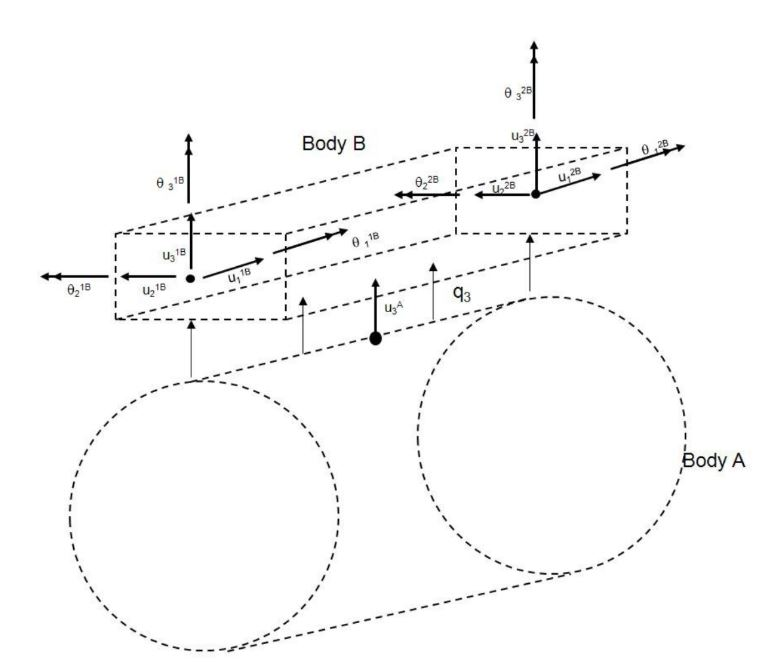
\includegraphics[scale=0.8]{figures/hcont463}
\caption[$\; \:$HCONT463]{Degrees of freedom for HCONT463, \cite{Bflextheory2013} }
 \label{fig:HCONT463}
\end{figure}

\subsubsection{HCONT454}
The purpose of the HCONT454 element is to connect two HSHEAR454 element groups (A and B) in the same layer by considering hoop contact between them and the reduction and expansion of gap due to curvature. Figure \ref{fig:HCONT4541} illustrates how the element was used in this study to describe the contact between the conductors in the cross-section.
\begin{figure}[H]
\centering
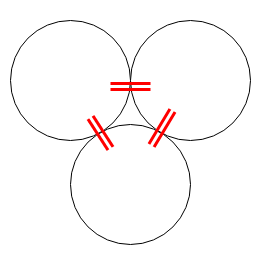
\includegraphics[scale=0.7]{figures/HCONT4541}
\caption[$\; \:$Illustration of HCONT454]{Illustration of HCONT454 connecting 3 conductors in a cable cross section}
 \label{fig:HCONT4541}
\end{figure}


The element has 36 degrees of freedom as can be seen in Figure \ref{fig:HCONT454},  where the extra 12 dofs are used to describe the beam strains of the center as this affect the gap in compression and tension. All three directions, $X^1$, $X^2$ and $X^3$ are included where the $X^2$ direction represents contact, and the others friction. The energy functional described for the HSHEAR463 element in Equations \ref{eq:energy} to \ref{eq:contact} are also valid for the HCONT454 element. The contact kinematics in the normal direction can be expressed as: 
\begin{equation}
    \Delta u_n=(\Delta \boldsymbol{u}_B-\Delta \boldsymbol{u}_A) \cdot \bold{n}=(\Delta \boldsymbol{u}_2^{0B}-\Delta \boldsymbol{u}_2^{0A}+\frac{b}{Ff}(\Delta \epsilon_\psi+\Delta \epsilon_{Z^1}))
\end{equation}
\noindent Where $ \Delta \epsilon_\psi$ is the hoop strain:
\begin{equation}
    \Delta \epsilon_\psi =\frac{\Delta u_3^{0A} + \Delta u_3^{0B}}{2R}
\end{equation}
and:
\begin{equation}
    \Delta \epsilon_{Z^1} = -R \sin \psi \Delta v_{,11} + R \cos \psi \Delta w_{,11}
\end{equation}
Where R is the mean helix radius of the two bodies and $v_{,11}$ and $w_{,11}$ are the center beam transverse curvatures differentiated  two times with respect to longitudinal direction. \\\\ The only contribution to the  incremental relative tangential displacement is from the helix side:
\begin{equation}
    \Delta u_s = (\Delta \boldsymbol{u}_B -\Delta \boldsymbol{u}_A) \cdot \bold{s}=(\Delta \boldsymbol{u}_1^{0B} -\Delta \boldsymbol{u}_1^{0B})
\end{equation}

\begin{equation}
    \Delta u_t = (\Delta \boldsymbol{u}_B -\Delta \boldsymbol{u}_A) \cdot \bold{t}=(\Delta \boldsymbol{u}_3^{0B} -\Delta \boldsymbol{u}_3^{0B})
\end{equation}. 

\begin{figure}[H]
\centering
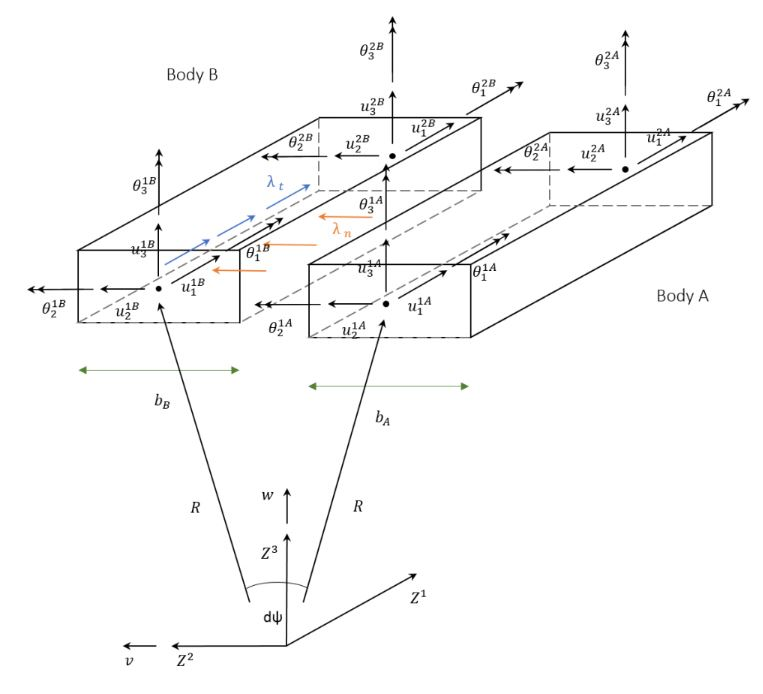
\includegraphics[scale=0.8]{figures/hcont454}
\caption[$\; \:$HCONT454]{Degrees of freedom for HCONT454, \cite{Bflextheory2017} }
 \label{fig:HCONT454}
\end{figure}

\subsubsection{PIPE52}
PIPE52 element is often used to model conic bend stiffeners. It supports a general description of flexible risers and is used to describe "pipe-in-pipe" with a non-linear elastic material curve. It has the same kinematics as PIPE31. 

\subsubsection{CONT130}
A three-node contact element often used to describe contact between a pipe inside a pipe. 







